% Created 2021-01-24 Sun 22:50
% Intended LaTeX compiler: pdflatex
\documentclass[11pt]{article}
\usepackage[utf8]{inputenc}
\usepackage[T1]{fontenc}
\usepackage{graphicx}
\usepackage{grffile}
\usepackage{longtable}
\usepackage{wrapfig}
\usepackage{rotating}
\usepackage[normalem]{ulem}
\usepackage{amsmath}
\usepackage{textcomp}
\usepackage{amssymb}
\usepackage{capt-of}
\usepackage{hyperref}
\usepackage{minted}
\hypersetup{colorlinks=true, linkcolor=black, filecolor=red, urlcolor=blue}
\usepackage[turkish]{babel}
\author{Eren Hatırnaz}
\date{15 Eylül 2019}
\title{Yazılım Gündemi - 9\\\medskip
\large 9-15 Eylül 2019}
\hypersetup{
 pdfauthor={Eren Hatırnaz},
 pdftitle={Yazılım Gündemi - 9},
 pdfkeywords={},
 pdfsubject={},
 pdfcreator={Emacs 27.1 (Org mode 9.3)},
 pdflang={Turkish}}
\begin{document}

\maketitle
\tableofcontents \clearpage\shorthandoff{=}

\begin{center}
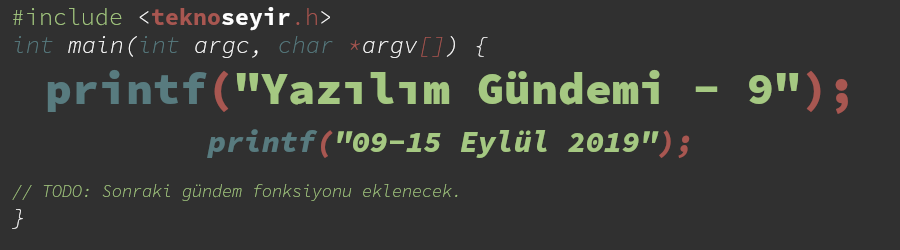
\includegraphics[width=.9\linewidth]{gorseller/yazilim-gundemi-banner.png}
\end{center}

\begin{center}
\href{../08/yazilim-gundemi-08.pdf}{< Önceki Gündem} | \textbf{9-15 Eylül 2019} | \href{../10/yazilim-gundemi-10.pdf}{Sonraki Gündem >}

\href{https://teknoseyir.com/blog/yazilim-gundemi-9-9-15-eylul-2019}{TeknoSeyir'de Oku}
\end{center}

\section{Python 2'nin \href{https://www.python.org/doc/sunset-python-2/}{3 aylık ömrü kalmış}}
\label{sec:org2f66379}
Bildiğiniz gibi Python programlama dili uzun bir süredir iki ayrı sürüm
üzerinden geliştirilmeye devam ediyor. Fakat Python 2.x numaralı sürümler için
yolun sonu gözüktü. Python takımı, 1 Ocak 2020'den itibaren Python 2 sürümünün
geliştirilmeye devam edilmediğini duyurdu. Buna güvenlik güncelleştirmeleri de
dahil. Yani Python 2 artık tamamen ölüyor.

Açıkcası pek üzüldüğümü söyleyemem. Yarattığı gereksiz "Python 2 mi, 3 mü?"
kafa karışıklığını da düşününce bu kadar uzun süre destek verilmesine bile
şaşırıyorum. Neyse, ölünün arkasından kötü konuşulmaz ama Python takımı \href{https://pythonclock.org/}{şöyle
bir web sitesi} açarak, Python 2 sürümünün ölüm gününe geri sayım başlatmış. Bu
biraz ağır olmuş sanki.

Python 2 ile yazılmış projelerinizi Python 3 sürümüne geçirmek için Python
takımı tarafından yayınlanan şu rehberi inceleyebilirsiniz: \href{https://docs.python.org/3/howto/pyporting.html}{Porting Python 2
Code to Python 3}. Son son helallik almayı da unutmayın Python 2'den.
\section{TypeScript 3.7 ile gelecek yenilikler}
\label{sec:org4c10f01}
5 Kasım'da \href{https://github.com/microsoft/TypeScript/issues/33352}{yayınlanması planlanan} TypeScript programlama dilinin 3.7 sürümü
ile gelecek olan birkaç özellik bu şekilde:

\subsection{\href{https://github.com/microsoft/TypeScript/issues/26578}{Null Coalescing}}
\label{sec:org6a723cb}
Bu özelliğin benzeri aslında JavaScript'in kendisinde mevcut fakat bazı
durumlarda sorun olabiliyor. Örneğin:
\begin{minted}[breaklines=true,breakanywhere=true,frame=lines, linenos, label=TypeScript, labelposition=topline]{typescript}
const final_sonuc = sonuc1 || sonuc2;
\end{minted}
gibi bir ifadede, \texttt{sonuc1} değişkeni eğer boş string ya da sıfır gibi \href{https://developer.mozilla.org/en-US/docs/Glossary/Falsy}{falsy}
ifadeler varsa, bunları tanımlı değildir olarak kabul edip \texttt{sonuc2}
değişkenini \texttt{sonuc\_final} 'e aktarabiliyordu.

TypeScript 3.7 ile gelecek olan \texttt{??} ifadesi ile bu sorunun önüne geçilmiş
oluyor. Şöyle ki:
\begin{minted}[breaklines=true,breakanywhere=true,frame=lines, linenos, label=TypeScript, labelposition=topline]{typescript}
const final_sonuc = sonuc1 ?? sonuc2;
\end{minted}
şeklinde kullanım sayesinde artık \texttt{sonuc1} değişkeni \href{https://developer.mozilla.org/en-US/docs/Glossary/Falsy}{falsy} ifadeler içerse
bile tanımlı olarak kabul edilecek, çünkü öyle bir değişken mevcut.
\subsection{\href{https://github.com/microsoft/TypeScript/issues/16}{Optional Chaining}}
\label{sec:org9e33b09}
Bu özellik sayesinde artık uzun ve iç içe if sorguları yapmak zorunda
kalmayacağız. Önceden şöyle uzun bir ifade ile yaptığımız şeyi:
\begin{minted}[breaklines=true,breakanywhere=true,frame=lines, linenos, label=TypeScript, labelposition=topline]{typescript}
let sonuc = veri ? (veri.anahtar1 ? veri.anahtar1.anahtar2 : undefined) : undefined;
\end{minted}
\texttt{veri.anahtar1.anahtar2} değerini getirmek için değişkenin tanımlı olmama
ihtimaline karşı böyle bir kullanım yapıyorduk.

Fakat artık bunu şu şekilde sadeleştirebileceğiz:
\begin{minted}[breaklines=true,breakanywhere=true,frame=lines, linenos, label=TypeScript, labelposition=topline]{typescript}
let sonuc = veri?.anathar1?.anahtar2;
\end{minted}

Yeni eklenecek diğer özellikler için \href{https://github.com/microsoft/TypeScript/issues/33352}{bu sayfaya} göz atabilirsiniz.
\section{Oracle, JDK indirmeleri için \href{https://www.oracle.com/java/technologies/jdk8-downloads.html}{artık üyelik istiyor}}
\label{sec:orge375fda}
Oracle elinde tuttuğu Java teknolojisinin suyunu sıkmaya devam ediyor. Şimdi de
lisans değişikliğine giderek, artık Java SE Development Kit indirmeleri için
üye olmayı zorunlu kıldı ve kişisel (ticari olmayan) projelerde kullanırken de
proje hakkında detayları istemeye başlayacakmış. Yani Oracle firması hoşuna
gitmeyen projelere JDK vermeyebilir. OpenJDK tarafında bir değişiklik yok, GPL
lisansı ile jdk.java.net adresi üzerinden dağıtılmaya devam ediyor.

Nedir bu Oracle'dan çektiğimiz?!
\section{Dünya Programcılar Günümüz kutlu olsun!}
\label{sec:orge41122f}
Her yılın 256'ıncı gününde kutlanan bir günümüz varmış, ben de yeni öğrendim.
256.gün olmasının nedeni de, hem 8-bit ile yazılabilecek toplam 256 sayı
olmasından (0 dahil), hem de 2'nin 365'den küçük en büyük katı olduğu içinmiş.
Bu yıl da 13 Eylül tarihine denk gelmiş. \href{https://www.youtube.com/watch?v=QsxbbHG7KT8}{O hale günümüz kutlu olsun arkadaşlar}
\section{Diğer Haberler}
\label{sec:org26263bd}
\begin{itemize}
\item GitHub, Rails 6.0 \href{https://github.blog/2019-09-09-running-github-on-rails-6-0/}{sürümüne geçtiğini duyurdu}.
\item MDN ve CanIUse \href{https://hacks.mozilla.org/2019/09/caniuse-and-mdn-compat-data-collaboration/}{güçlerini birleştirdi}.
\item Google, JavaScript ve WebAssembly motoru V8'in \href{https://v8.dev/blog/v8-lite}{daha hafif bir versiyonu
üzerinde çalışıyormuş}: \href{https://docs.google.com/document/d/10qh2-b4C5OtSg-xLwyZpEI5ZihVBPtn1xwKBbQC26yI/edit}{V8 Lite}.
\item Django 3.0 \href{https://www.djangoproject.com/weblog/2019/sep/10/django-30-alpha-1-released/}{alpha 1 sürümü} duyuruldu.
\item C++20 konseptleri Visual Studio 2019 \href{https://devblogs.microsoft.com/cppblog/c20-concepts-are-here-in-visual-studio-2019-version-16-3/}{16.3 Preview 2 sürümünde kullanılabilir
olmuş}.
\item C++ kütüphane yöneticisi \href{https://github.com/microsoft/vcpkg}{vcpkg} aracının \href{https://github.com/microsoft/vcpkg/releases/tag/2019.08}{2019.08 sürümü yayınlandı}.
\item Stripe komut satırı aracını (CLI) \href{https://twitter.com/stripe/status/1171474829570035712}{açık kaynak olarak yayınladı}, \href{https://github.com/stripe/stripe-cli}{GitHub
Deposu}.
\item PHP mail gruplarında \href{https://externals.io/message/106963}{hararetli tartışmalar devam ediyor}.
\item Dart programlama dili \href{https://medium.com/dartlang/announcing-dart-2-5-super-charged-development-328822024970}{2.5 sürümünü duyurdu}.
\item Bulut uygulamaları için özelleştirilmiş yeni bir açık kaynak programlama
dili duyuruldu: \href{https://v1-0.ballerina.io/}{Ballerina}, \href{https://github.com/ballerina-platform}{GitHub Sayfası}.
\item Yeni bir proje yönetim \href{https://techcrunch.com/2019/09/10/clubhouse-announces-new-collaboration-tool-and-free-version-of-its-project-management-platform/}{platformu duyuruldu}: \href{https://clubhouse.io/}{Clubhouse}.
\item Eclipse organizasyonu, \href{https://jakarta.ee/}{Jakarta EE 8} projesini \href{https://www.zdnet.com/article/java-finally-goes-all-in-on-open-source-with-the-release-of-jakarta-ee-8/}{açık kaynak olarak kullanıma
açtı}.
\item Dağıtık log sistemi \href{https://wecode.wepay.com/posts/waltz-a-distributed-write-ahead-log}{Waltz} açık kaynak olarak duyuruldu. \href{https://github.com/wepay/waltz}{GitHub Deposu}
\item Captcha alternatifi bir girişim: \href{https://wehatecaptchas.com/}{WeHateCaptchas}.
\item Netlify, FaunaDB için \href{https://www.netlify.com/blog/2019/09/10/announcing-the-faunadb-add-on-for-netlify/}{eklentisini duyurdu}.
\item Yazı sınıflandırma kütüphanesi cherry, \href{https://github.com/Windsooon/cherry/releases/tag/v2.0}{2.0 sürümünü duyurdu}.
\item Nestedj \href{https://github.com/eXsio/nestedj/releases/tag/4.0.0}{4.0.0 sürümü çıktı}.
\end{itemize}
\section{Lisans}
\label{sec:org0c39b92}
\begin{center}
\begin{center}

\includegraphics[height=1.5cm]{../../../img/CC_BY-NC-SA_4.0.png}
\end{center}

\href{yazilim-gundemi-09.pdf}{Yazılım Gündemi - 9} yazısı \href{https://erenhatirnaz.github.io}{Eren Hatırnaz} tarafından \href{http://creativecommons.org/licenses/by-nc-sa/4.0/}{Creative Commons
Atıf-GayriTicari-AynıLisanslaPaylaş 4.0 Uluslararası Lisansı} (CC BY-NC-SA 4.0)
ile lisanslanmıştır.
\end{center}
\end{document}
